\documentclass{article}
\usepackage{graphicx,fancyhdr,amsmath,amssymb,amsthm,subfig,url,hyperref}
\usepackage[margin=1in]{geometry}

\usepackage{natbib}
\usepackage{cancel}

\usepackage{minted}

\usepackage[shortlabels]{enumitem}

%----------------------- Macros and Definitions --------------------------

%%% FILL THIS OUT
\newcommand{\studentname}{Jane Doe}
\newcommand{\suid}{janedoe}
\newcommand{\exerciseset}{Homework}
%%% END



\renewcommand{\theenumi}{\bf \Alph{enumi}}

\theoremstyle{plain}
\newtheorem{theorem}{Theorem}
\newtheorem{lemma}[theorem]{Lemma}


\graphicspath{{figures/}}

%-------------------------------- Title ----------------------------------

\title{Study Kasus 3: \textit{Catalan Number}} 
\author{IN232 Matematika Diskrit}
\date{}
%--------------------------------- Text ----------------------------------

\begin{document}
\maketitle

%	\begin{enumerate}[-,topsep=0pt, nosep,label=\alph*. ]
%		\item How many ways are there to pick two representatives, so that one is a mathematics major and the other is a computer science major?
%		\item How many ways are there to pick one representative who is either a mathematics major or a computer science major?
%	\end{enumerate}

\section*{Menghitung Rute dari Kotak Persegi}
Ada berapa rute dari titik paling kiri bawah kotak persegi $n \times n$ ke titik paling kanan atas jika anda dibatasi untuk bepergian hanya ke kanan atau ke atas? Salah satunya rute (berwarna \textcolor{blue}{biru}) ditunjukkan dalam kotak $4 \times 4$ pada Figure \ref{fig:4-by-4-grid}.

\begin{figure}[!ht]
	\centering
	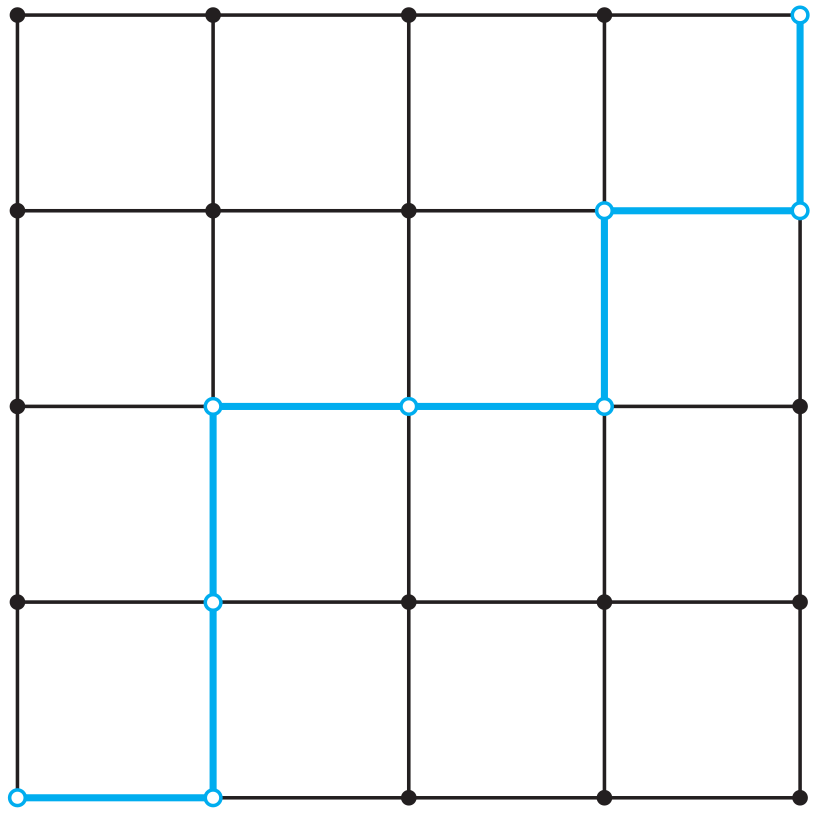
\includegraphics[scale=.225]{images/4-by-4-grid}
	\caption{Kotak $4 \times 4$ dengan satu rute yang diwarnai biru \citep{johnsonbaugh2009discrete}}
	\label{fig:4-by-4-grid}
\end{figure}

\section*{Modifikasi dari Kasus Sebelumnya}
Ada berapa rute dari titik paling kiri bawah dari kotak persegi $n \times n$ ke titik paling kanan atas jika anda dibatasi untuk bepergian hanya ke kanan atau ke atas dan jika anda diperbolehkan untuk menyentuh tetapi tidak melewati garis diagonal dari titik paling kiri bawah ke titik paling kanan atas?

\section*{Catalan Number}
	\begin{enumerate}[-,topsep=0pt, nosep,label=\alph*. ]
		\item Apakah \textit{Catalan number} atau bilangan \textit{Catalan} itu?
		\item Kaitkan \textit{Catalan number} dengan kasus modifikasi sebelumnya.
	\end{enumerate}



%
%\section*{Implementasi}
%	\begin{enumerate}[-,topsep=0pt, nosep,label=\arabic*. ]
%		\item Ubahlah relasi rekurensi di Persamaan \eqref{eq:price-recursive-relation} menjadi \textit{solusi eksplisit}.  
%		\item Implementasi Persamaan \eqref{eq:price-recursive-relation} dalam program.
%	\end{enumerate}
%
%\begin{minted}{python}
%def compute_cobweb(p_0, a, b, k, n):
%    """
%    Compute a price at n based on cobweb recursive relation	
%    
%    Parameters:
%    -----------
%    p_0 : float
%        An initial price
%    
%    a, b, k : float
%        Three positive parameters
%    
%    n : int
%        The final time for the price to be computed    
%    
%    Returns:
%    --------
%    p_n : float
%        The final price at time n
%    """
%    pass
%\end{minted}
%
%\noindent Sebagai test drive, silakan anda hitung secara manual dan bandingkan hasil manual dengan hasil program.


\bibliographystyle{apalike}
\bibliography{references}


\end{document}
